\section{Introduction}
``Programming by demonstration (PbD) has become a central topic of robotics and spans across general research areas such as human-robot interaction, machine learning, machine vision and motor control" (\cite{billard2008robot}).
 possess the robot programming knowledge, to communicate skills to robots more easily.
The underlying concept is to learn a new skill from a set of correct demonstrations, thus reducing the complexity of the search space and accelerating learning.
It offers a framework for service robotics applications, independent of the robot platform, and reduces the overhead of reprogramming the robot for different tasks.

The problem of learning a skill can be considered as learning a function that maps a world state to an action.
 In real-world applications, states can only be partially observed due to restricted sensor availability.
 Hence, we assume that the robot learner has access to the observed state $Z$ instead.
 A function $\pi : Z \rightarrow A$, referred to as a \textit{policy}, allows the robot to select actions from an action domain $A$, given observations of the world state.
 
Programming by demonstration is an approach to learn this policy from demonstration data, known as \textit{examples}.
% ``Examples are sequences of state-action pairs that are recorded during the teacher's demonstration of the desired robot behaviour." \cite{argall2009survey} 
Unlike learning techniques in reinforcement learning, PbD is aimed at learning from correct examples only.
 Thus, PbD can be seen as a subset of Supervised Learning, as the agent is presented with labeled training data and tries to learn an approximation of the function, which produced the data (\cite{argall2009survey}).

 \cite{nicolescu2003natural} present a PbD approach, which allows the robot to learn skill representations and refine them by using feedback cues provided by the teacher.
 Similarly, \cite{calinon2007active} and \cite{calinon2007incremental} implement systems, which actively involve the teacher in the robot's learning process, by providing human guidance to a humanoid robot.
 The robot first observes the demonstration performed by the teacher, who is wearing motion sensors.
 When it tries to reproduce the action, the teacher can refine the movement by physically moving its limbs.

\section{Design choices}\label{subsec:Design choices}
There are different design choices to consider when developing a new PbD system.
We differentiate between the choice of the demonstrator (human or robot), in particular who controls the demonstration and who executes the demonstration.
Consider the example of a simple pick up action of an object.
The teacher could be demonstrating the action using their own hands, while the robot observes the motion, or by moving the robot's joints directly.
Furthermore, the state and action can either be represented in a discrete way (\textit{``object on the table"} or \textit{``robot holding object"}) or in a continuous way using the 3D positions of the robot's end effector and the box.
There is also the choice of the demonstration technique, i.e. whether the data is provided to the learner incrementally or once all data has been gathered.
 
Despite the different design choices, there are common aspects across all PbD applications. 
Firstly, the teacher demonstrates the desired behaviour and, secondly, the learner derives a policy from this set of demonstrations to reproduce the behaviour.

%Building the data set
\section{Gathering demonstrations} \label{subsec:Gathering demonstrations}
%There are many ways for the robot to collect data.
% We differentiate between:
%\begin{itemize}
%    \item How much data is collected at a time: incremental vs batch learning
%    \item Who provides the data: robot can look for data on its own or it is provided data by user
%    \item Which interaction modalities are used: vision, voice or touch. 
%\end{itemize}

There exist various techniques for gathering demonstration examples.
 We differentiate between methods for action recording and action execution.
 Consider the two mappings (\cite{argall2009survey}):
\begin{itemize}
\item Record mapping $g_R(z,a)$: A mapping between the exact actions demonstrated by the teacher and those recorded within the dataset.
\item Embodiment mapping $g_E(z,a)$: A mapping between the actions recorded in the dataset and the actions executed by the robot learner.
\end{itemize}
If the teacher manipulates the robot's arm to demonstrate the desired behaviour and the joint trajectories are recorded, then the record mapping is the identity function ($g_R(z,a) = I(z,a)$).
 Otherwise, the teacher information is encoded and recorded into the dataset according to a mapping function ($g_R(z,a) \neq I(z,a))$.
 Take as an example a human teacher, who demonstrates the action of moving an object on the table using their own hand.
 The robot records the movement using its camera and tries to extract the necessary information to perform this action, while the teacher's actual joint movements remain unknown.
 Thus, the recorded dataset is extracted from the camera images using the record mapping.

Similarly, for the action execution, if the recorded actions in the dataset are executed directly by the robot learner, the embodiment mapping is the identity function ($g_E(z,a) = I(z,a)$).
 Otherwise, it is a function $g_E(z,a) \neq I(z,a)$, which translates the recorded data for the robot learner.
  We refer to the two different action execution methods as \textit{Demonstration} and \textit{Imitation} respectively.
When dealing with real robots, the embodiment mapping is particularly important, as the teacher's demonstration is executed in a physical environment, rather than a simulated one.
 Successful learning of the action will depend on an accurate mapping between the recorded dataset and the learner's movement capabilities.
  \begin{figure}[!h]
    \centering
    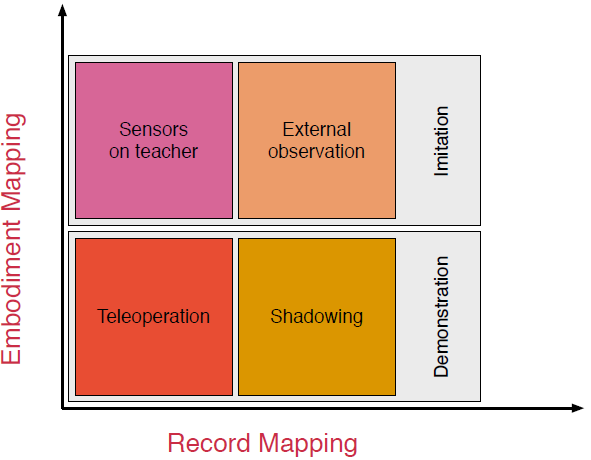
\includegraphics[scale=0.5]{figures/Gathering}
    \caption{Intersection of the record and embodiment mappings.}
    \label{fig:Gathering demonstrations}
  \end{figure}

Given the above mappings and categorisations, we differentiate between four data acquisition approaches, depending on whether the record or embodiment mappings are equal to the identity function or not (see also Figure \ref{fig:Gathering demonstrations}):

\begin{itemize}
\item Teleoperation ($g_R(z,a) = I(z,a)$ and $g_E(z,a) = I(z,a)$): The teacher operates the robot learner platform, while the robot's sensors record the task execution of its own joints.
\item Shadowing ($g_R(z,a) \neq I(z,a)$ and $g_E(z,a) = I(z,a)$): The teacher demonstrates tasks using their own hands, while the robot learner records the execution and tries to mimic the teacher's task execution.
\item Sensors on teacher  ($g_R(z,a) = I(z,a)$ and $g_E(z,a) \neq I(z,a)$): The teacher wears sensors, which record the task execution.
 The robot learner needs to translate the teacher's joint positions for its own task execution.
\item External observation  ($g_R(z,a) \neq I(z,a)$ and $g_E(z,a) \neq I(z,a)$): The teacher executes the tasks using their own hands, while external sensors, that may or may not be on the robot learner, are used to record the teacher's task execution.
\end{itemize}

A full categorisation for building the demonstration dataset is shown in Figure \ref{fig:Gathering demonstrations2}.
 The use of intermediate mappings can lead to a loss of information of the demonstrated actions.
 Teleoperation is the most accurate way to transfer the teacher's intention to the robot, as the exact actions are recorded and executed without any intermediate translations.
 The choice for gathering demonstration data depends highly on the robot's sensory capabilities and the complexity of the demonstrated task.
 If the robot's joints do not correspond to those of the teacher, it is difficult to find an accurate mapping.
 For the implementation of our framework, we decided to take a teleoperation approach.
 The teacher will be handling the robot's limb directly, when demonstrating the task, while the robot records its own joint movements.

  \begin{figure}[ht]
    \centering
    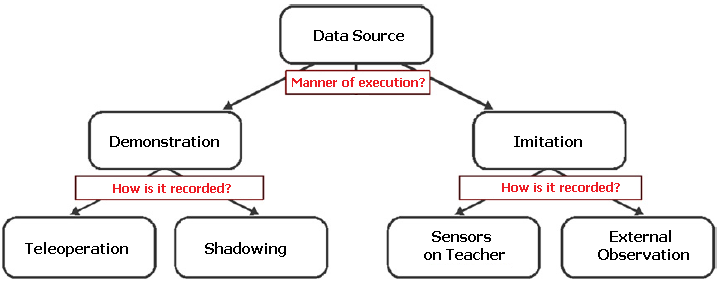
\includegraphics[scale=0.6]{figures/Gathering3}
    \caption{Typical approaches to providing demonstrations (\cite{argall2009survey})}
    \label{fig:Gathering demonstrations2}
  \end{figure}


